\begin{frame}{$\chi_{b1,2}(1,2,3P) \to \OneS \gamma$ fit model (1)}

\centering
\setlength{\unitlength}{1mm}
\resizebox{.7\textwidth}{!}{
\begin{picture}(50,40)
  %
\put(0,0){
  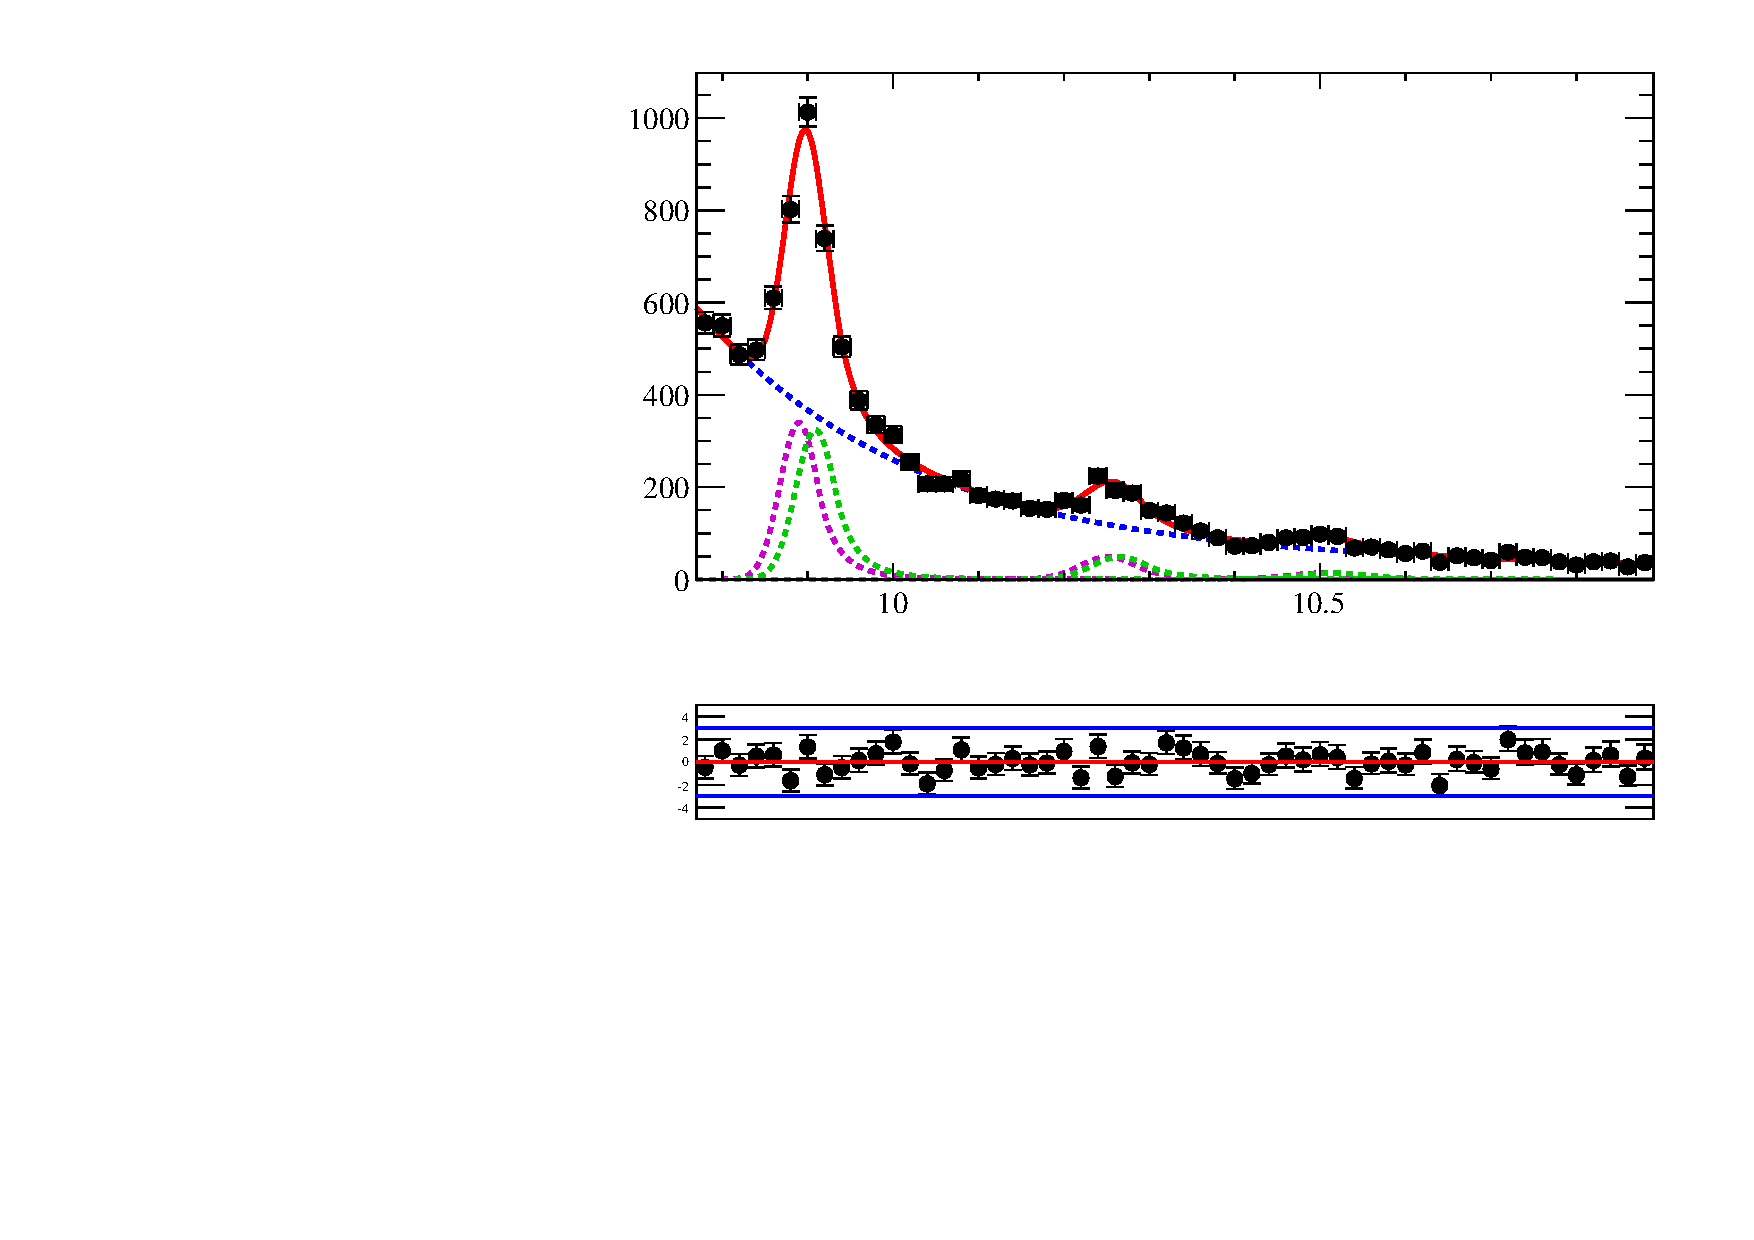
\includegraphics[width=50mm, height=40mm]{chib_f2011_14_40}
}

\put(0,15){\tiny \begin{sideways}Candidates/(20\mevcc)\end{sideways}}
\put(5,9){\tiny $m_{\mumu \gamma} - m_{\mumu} + m_{\Y1S}^{PDG} \left[\gevcc\right]$}
\put(30,35){\footnotesize $\sqrt{s} = 7\tev$}

\put(15,35){\tiny \chibOneP}
\put(25,20){\tiny \chibTwoP}
\put(35,17){\tiny \chibThreeP}

\put(9,17){\scalebox{0.4}{$\chi_{b1}$}}
\put(14.5,17){\scalebox{0.4}{$\chi_{b2}$}}
   

% \graphpaper[5](0,0)(50, 40)        
\end{picture}
}

\begin{itemize}
\item One Crystal Ball (CB) for each $\chi_{b1,2}(1P,2P,3P)$ state: 6 CB in total
\item Exclude the study of $\chi_{b0}$ due to its low radiative branching ratio.
\item Product of exponential and linear combination of 
polynomials  for combinatorial background.
\end{itemize}

\end{frame}
